\documentclass[tikz, border=10pt]{standalone}
\usepackage{tikz}
\usepackage{xcolor}
\usepackage{amssymb}
\usepackage{marvosym}
\usetikzlibrary{shapes.geometric, arrows.meta, positioning, fit, backgrounds, shadows}

% ── Colour palette ────────────────────────────────────────────────────────────
\definecolor{halBlue}   {RGB}{30,  90, 160}
\definecolor{halCyan}   {RGB}{  0, 160, 200}
\definecolor{halGreen}  {RGB}{ 30, 150,  80}
\definecolor{halOrange} {RGB}{220, 120,  30}
\definecolor{halRed}    {RGB}{190,  50,  50}
\definecolor{halGray}   {RGB}{240, 240, 245}
\definecolor{halDarkGray}{RGB}{80,  80,  90}

% ── TikZ styles ───────────────────────────────────────────────────────────────
\tikzset{
  %% file node (rounded rect, light fill)
  filenode/.style={
    rectangle, rounded corners=6pt,
    draw=#1!70!black, fill=#1!15,
    text=black, font=\sffamily\small\bfseries,
    minimum width=2.2cm, minimum height=0.8cm,
    drop shadow, align=center
  },
  %% pass box (larger, darker)
  passbox/.style={
    rectangle, rounded corners=4pt,
    draw=#1!80!black, fill=#1,
    text=white, font=\sffamily\bfseries\small,
    minimum width=3.6cm, minimum height=1.0cm,
    drop shadow, align=center
  },
  %% table box
  tablebox/.style={
    rectangle, rounded corners=4pt,
    draw=halDarkGray!60, fill=halGray,
    text=halDarkGray, font=\sffamily\footnotesize,
    minimum width=2.6cm, minimum height=0.75cm,
    align=center
  },
  %% arrow style
  myarrow/.style={
    -Stealth, line width=1.6pt, color=#1
  },
  %% thin dashed arrow
  dasharrow/.style={
    -Stealth, dashed, line width=1pt, color=halDarkGray!70
  },
  %% label on arrow
  arrlabel/.style={
    font=\sffamily\tiny\itshape, text=halDarkGray,
    fill=white, inner sep=1pt
  },
}

\begin{document}
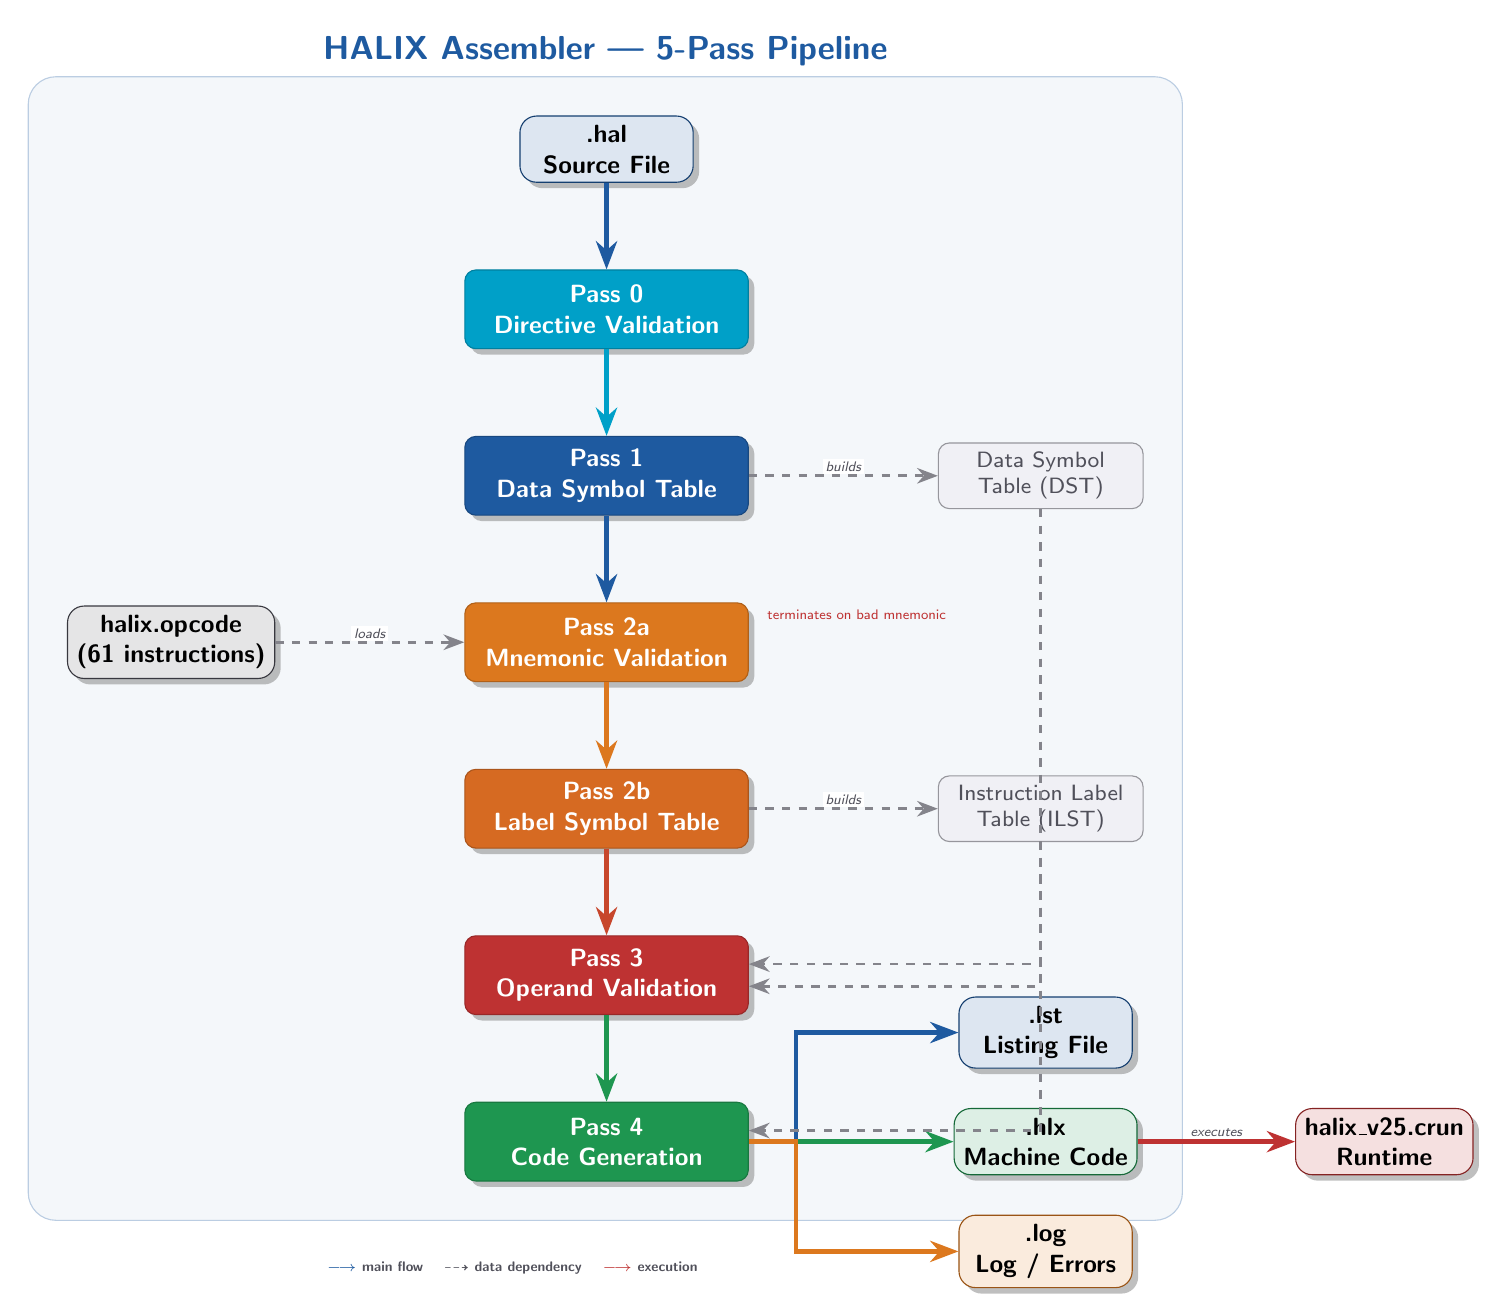
\begin{tikzpicture}[node distance=1.1cm and 2.2cm]

%% ════════════════════════════════════════════════════════
%%  INPUT FILE
%% ════════════════════════════════════════════════════════
\node[filenode=halBlue] (input) {.hal\\Source File};

%% ════════════════════════════════════════════════════════
%%  PASS NODES  (vertical stack, left column)
%% ════════════════════════════════════════════════════════
\node[passbox=halCyan,   below=of input]               (p0)  {Pass 0\\Directive Validation};
\node[passbox=halBlue,   below=of p0]                  (p1)  {Pass 1\\Data Symbol Table};
\node[passbox=halOrange, below=of p1]                  (p2a) {Pass 2a\\Mnemonic Validation};
\node[passbox=halOrange!80!halRed, below=of p2a]       (p2b) {Pass 2b\\Label Symbol Table};
\node[passbox=halRed,    below=of p2b]                 (p3)  {Pass 3\\Operand Validation};
\node[passbox=halGreen,  below=of p3]                  (p4)  {Pass 4\\Code Generation};

%% ════════════════════════════════════════════════════════
%%  OUTPUT FILES  (right of pass 4)
%% ════════════════════════════════════════════════════════
\node[filenode=halGreen,  right=2.6cm of p4]           (hlx) {.hlx\\Machine Code};
\node[filenode=halBlue,   above=0.5cm of hlx]          (lst) {.lst\\Listing File};
\node[filenode=halOrange, below=0.5cm of hlx]          (log) {.log\\Log / Errors};

%% ════════════════════════════════════════════════════════
%%  SYMBOL TABLES  (right of pass 1 and pass 2b)
%% ════════════════════════════════════════════════════════
\node[tablebox, right=2.4cm of p1]   (dst)  {Data Symbol\\Table (DST)};
\node[tablebox, right=2.4cm of p2b]  (ilst) {Instruction Label\\Table (ILST)};

%% ════════════════════════════════════════════════════════
%%  OPCODE CONFIG  (left of pass 2a)
%% ════════════════════════════════════════════════════════
\node[filenode=halDarkGray, left=2.4cm of p2a] (opcode) {halix.opcode\\(61 instructions)};

%% ════════════════════════════════════════════════════════
%%  RUNTIME  (right of hlx)
%% ════════════════════════════════════════════════════════
\node[filenode=halRed, right=2.0cm of hlx] (crun) {halix\_v25.crun\\Runtime};

%% ════════════════════════════════════════════════════════
%%  MAIN PIPELINE ARROWS
%% ════════════════════════════════════════════════════════
\draw[myarrow=halBlue]   (input) -- (p0);
\draw[myarrow=halCyan]   (p0)    -- (p1);
\draw[myarrow=halBlue]   (p1)    -- (p2a);
\draw[myarrow=halOrange] (p2a)   -- (p2b);
\draw[myarrow=halRed!70!halOrange] (p2b) -- (p3);
\draw[myarrow=halGreen]  (p3)    -- (p4);

%% output arrows
\draw[myarrow=halGreen]  (p4) -- (hlx);
\draw[myarrow=halBlue]   (p4.east) -- ++(0.6,0) |- (lst.west);
\draw[myarrow=halOrange] (p4.east) -- ++(0.6,0) |- (log.west);

%% symbol table production arrows
\draw[dasharrow] (p1)  -- node[arrlabel,above]{builds} (dst);
\draw[dasharrow] (p2b) -- node[arrlabel,above]{builds} (ilst);

%% symbol table consumption arrows (dashed, from p3/p4)
\draw[dasharrow] (dst.south)  |- ([yshift=4pt]p3.east);
\draw[dasharrow] (ilst.south) |- ([yshift=-4pt]p3.east);
\draw[dasharrow] (dst.south)  |- ([yshift=4pt]p4.east);

%% opcode file arrow
\draw[dasharrow] (opcode) -- node[arrlabel,above]{loads} (p2a);

%% runtime arrow
\draw[myarrow=halRed] (hlx) -- node[arrlabel,above]{executes} (crun);

%% ════════════════════════════════════════════════════════
%%  ERROR TERMINATION NOTE on pass boxes
%% ════════════════════════════════════════════════════════
\node[font=\sffamily\tiny, text=halRed, right=0.05cm of p2a, yshift=0.35cm]
  {$\lightning$ terminates on bad mnemonic};

%% ════════════════════════════════════════════════════════
%%  BACKGROUND PANEL
%% ════════════════════════════════════════════════════════
\begin{scope}[on background layer]
  \node[fill=halBlue!5, draw=halBlue!30, rounded corners=10pt,
        fit=(input)(p0)(p1)(p2a)(p2b)(p3)(p4)(dst)(ilst)(opcode),
        inner sep=14pt, label={[font=\sffamily\bfseries\large,
        text=halBlue]above:HALIX Assembler — 5-Pass Pipeline}] {};
\end{scope}

%% ════════════════════════════════════════════════════════
%%  LEGEND
%% ════════════════════════════════════════════════════════
\node[font=\sffamily\tiny\bfseries, text=halDarkGray,
      below=0.9cm of p4, xshift=-1.2cm] (leg)
  {\textcolor{halBlue}{$\longrightarrow$} main flow \quad
   \textcolor{halDarkGray}{$\dashrightarrow$} data dependency \quad
   \textcolor{halRed}{$\longrightarrow$} execution};

\end{tikzpicture}
\end{document}
